\documentclass{article}
\usepackage{graphicx} % Used to show UML model in eps
\usepackage{datetime} % Used to format time in LaTeX
\settimeformat{hhmmsstime} % The format we use for time 
\setlength{\parskip}{\baselineskip} % Put exactly one line between paragraphs
\setlength{\parindent}{0pt} % Do not indent paragraphs

\begin{document}
\title{TBA Gate Model Assignment}
\author{Joris Slob}
\date{October 2014}
\maketitle

\section{Introduction}

For a job application at TBA, I was given an exercise to show my
technical skills. The precise description of the exercise can be found
in ASSIGNMENT.md. In this report, I will describe my general approach
to this exercise.

\section{Estimation on paper}

To determine the approach I would take I first did some simple
calculations to see what I could expect. For this I took the xlsx file
and quick estimate of the solution.

First observation is that the entries in the xlsx file are all for one
day. The first truck arrives at the harbor at $T_1 =
\mbox{\formattime{6}{2}{29}}$ and the last truck arrives at $T_{1327}
= \mbox{\formattime{15}{24}{16}}$. That means that 1327 trucks arrive
in 561.78 minutes for an average of 2.36 trucks/min.

To deal with this load every part of the harbor has to be able to deal
with this rate of trucks. The entry gate takes 3 minutes on average to
deal with a truck, so to handle 2.36 trucks/min requires
$\frac{2.36}{1/3} = 7.08$ lanes.

The stack modules take 2 minutes on average to deal with trucks and
there are ten, so they can handle 5 trucks/min. We expect no problems
for this estimate there.

The exit gate takes 1 minute on average to deal with a truck, so to
handle the 2.36 trucks/min requires 2.36 lanes.

Let us model this gate problem in software to verify these results.

\section{Software model}

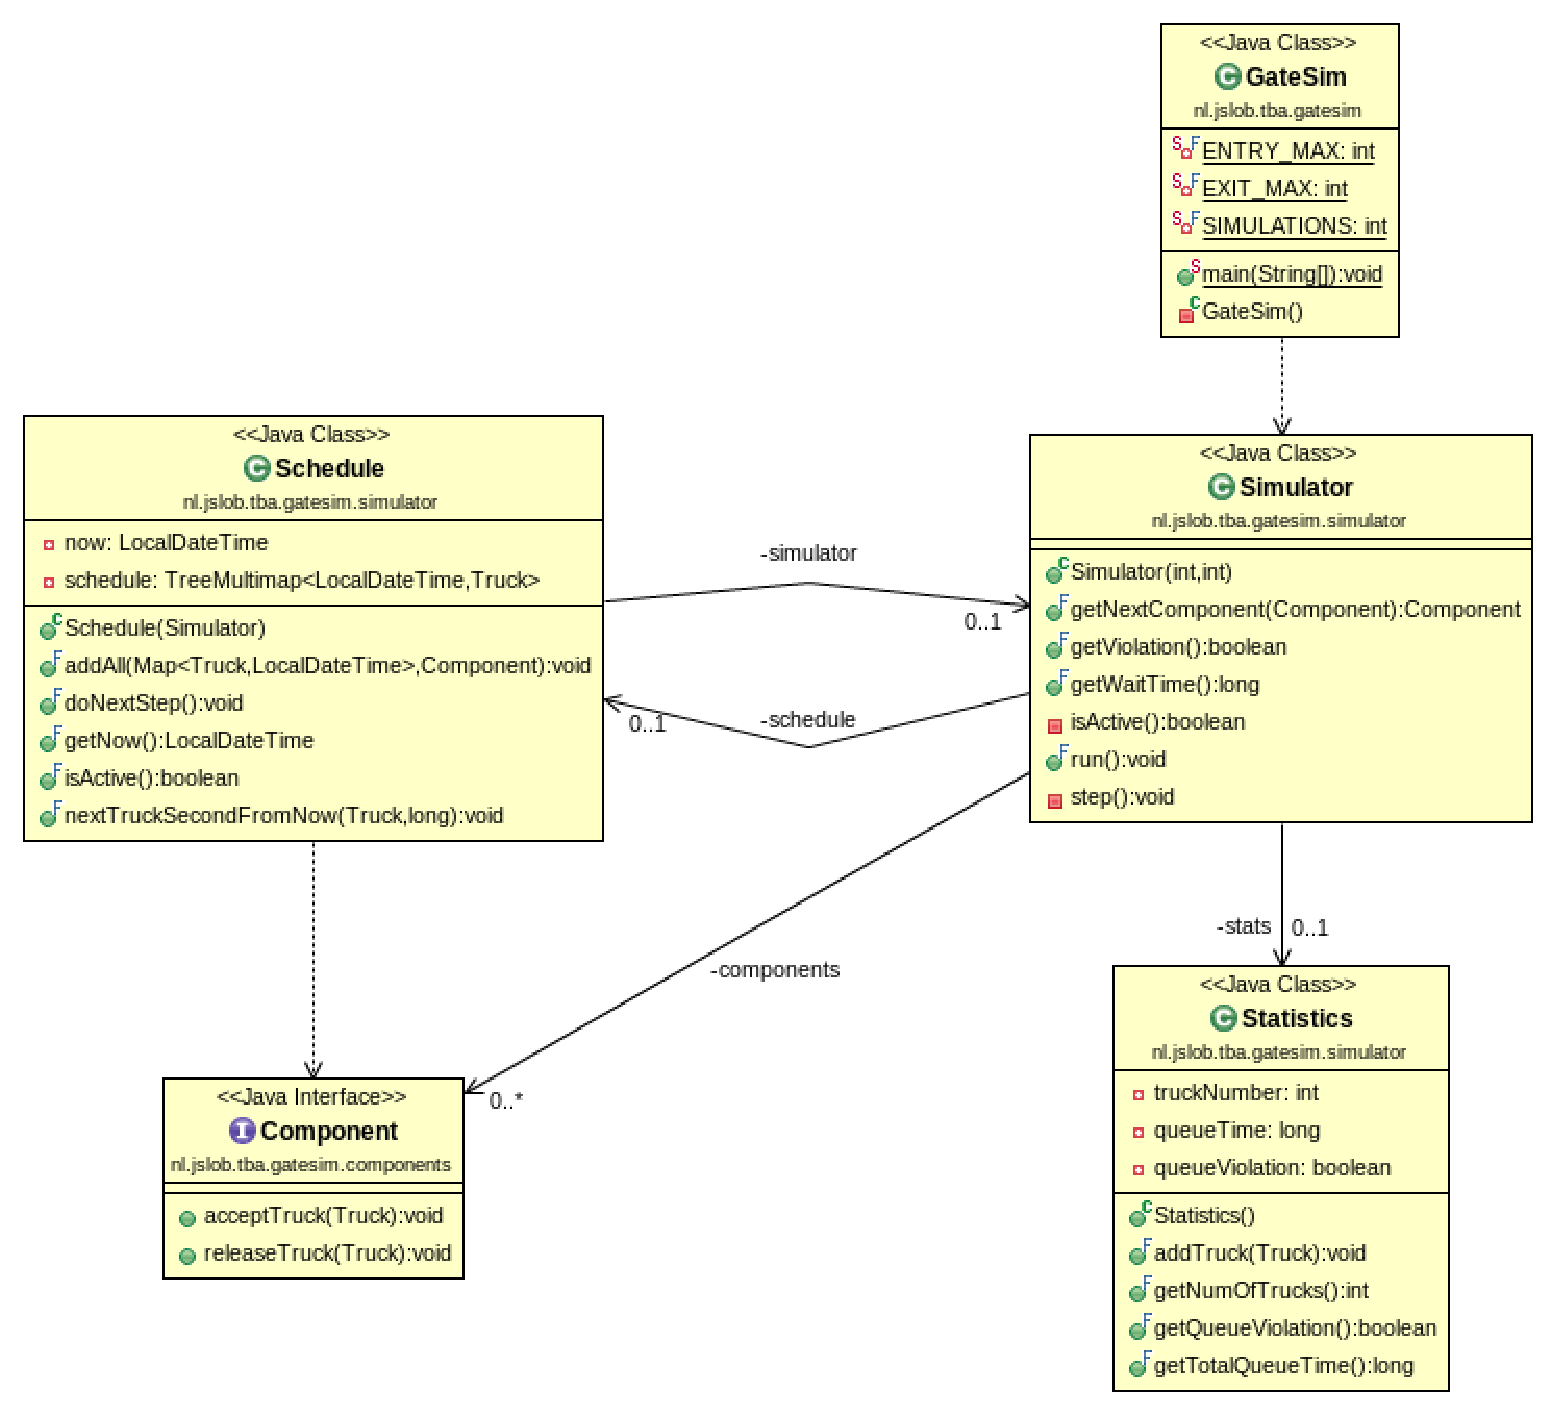
\includegraphics[scale=0.4]{Simulator.eps}

\section{Results}

The first result that satisfies the assignment is the model with 7
entry lanes and 3 exit lanes. This comes close to the initial estimate
given in the introduction. In this assignment we have introduced
another metric to evaluate the performance of the system:
TotalQueueTime. With data on the total time lost in queues the harbor
can consider opening more lanes to compensate truck waiting
time. Opening new lanes and operating them also has a cost, but these
were not given in the assignment.

This simulation is embarrassingly parallel and could be made to run
several simulations in separate threads.

\end{document}
